% Contributions are much appreciated, in order to contribute to this project, head over to this repository:
% https://github.com/bshramin/uofa-eng-assignment

\documentclass[11pt,letterpaper]{article}
\textwidth 6.5in
\textheight 9.in
\oddsidemargin 0in
\headheight 0in
\usepackage{graphicx}
\usepackage{fancybox}
\usepackage[utf8]{inputenc}
\usepackage{epsfig,graphicx}
\usepackage{multicol,pst-plot}
\usepackage{pstricks}
\usepackage{amsmath}
\usepackage{amsfonts}
\usepackage{amssymb}
\usepackage{eucal}
\usepackage[left=2cm,right=2cm,top=2cm,bottom=2cm]{geometry}
\usepackage{esvect}
\pagestyle{empty}
\DeclareMathOperator{\tr}{Tr}
\newcommand*{\op}[1]{\check{\mathbf#1}}
\newcommand{\bra}[1]{\langle #1 |}
\newcommand{\ket}[1]{| #1 \rangle}
\newcommand{\braket}[2]{\langle #1 | #2 \rangle}
\newcommand{\mean}[1]{\langle #1 \rangle}
\newcommand{\opvec}[1]{\check{\vec #1}}
\renewcommand{\sp}[1]{$${\begin{split}#1\end{split}}$$}

\usepackage{lipsum}

\usepackage{listings}
\usepackage{color}
\usepackage{wrapfig}
\usepackage[shortlabels]{enumitem}

\definecolor{codegreen}{rgb}{0,0.6,0}
\definecolor{codegray}{rgb}{0.5,0.5,0.5}
\definecolor{codepurple}{rgb}{0.58,0,0.82}
\definecolor{backcolour}{rgb}{0.95,0.95,0.92}

\lstdefinestyle{mystyle}{
	backgroundcolor=\color{backcolour},   
	commentstyle=\color{codegreen},
	keywordstyle=\color{magenta},
	numberstyle=\tiny\color{codegray},
	stringstyle=\color{codepurple},
	basicstyle=\footnotesize,
	breakatwhitespace=false,         
	breaklines=true,                 
	captionpos=b,                    
	keepspaces=true,                 
	numbers=left,                    
	numbersep=5pt,                  
	showspaces=false,                
	showstringspaces=false,
	showtabs=false,                  
	tabsize=2
}

\lstset{style=mystyle}

\begin{document}
\pagestyle{plain}

\begin{flushleft}
Estudiante: Fabio Quimbay\\
Email: fabio.quimbay883@comunidadunir.net\\
Profesor: Miguel Ángel Cabeza\\
Fecha: Noviembre 10 de 2022\\
\end{flushleft}

\begin{flushright}\vspace{-20mm}

\includegraphics[height=2cm]{logo.png}
\end{flushright}
 
\begin{center}\vspace{0cm}
\textbf{\large PER5786 2022-2023  Física 1 (GFI) - PER5786 2022-2023}\\
 Tema 3 - Movimientos elementales
\end{center}

 
\rule{\linewidth}{0.1mm}
%%%%%%%%%%%%%%%%%%%%%%%%%%%%%%%%%%%%%%%%%%%%%%%%%%%%%%%%%%%%%%%%%%%%%%%%

\bigskip
\bigskip

%%%%%%%%%%%%%%%%%%%%
\textbf{Problema propuesto 2}\\

\begin{wrapfigure}{r}{0.25\textwidth}
\begin{center}
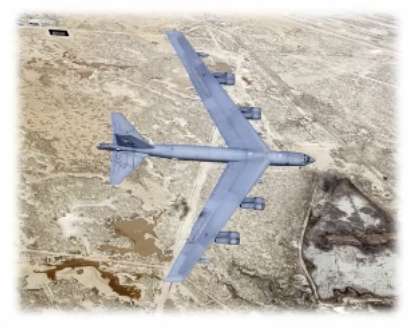
\includegraphics[width=0.25\textwidth]{problema_2.png}
\end{center}
\end{wrapfigure}

Un avión de bombardeo se dirige en línea recta hacia su objetivo a una velocidad de 900 km/h y a una altura de 8400 m. En el objetivo hay cañones antiaéreos cuyos proyectiles tienen una velocidad inicial de 600 m/s y el ángulo máximo de tiro es de 60 grados sobre la horizontal.\\

Prescindiendo del rozamiento del aire, se pide:

\begin{itemize}
  \item ¿A qué distancia horizontal del objetivo debe dejar caer las bombas el avión?
  \item ¿Cuánto tiempo antes de sobrevolar el objetivo debe liberar las bombas?
  \item ¿Puede ser derribado el avión por la defensa antiaérea?
\end{itemize}

\textbf{Formulas base:}\\

Se tomarán las siguientes formulas base del MRUA:

\begin{align}
\boxed{ V = V_{0} + a \cdot (t - t_{0})^2}\\
\boxed{ e = e_{0} + V_{0} \cdot (t - t_{0}) + \frac{1}{2} \cdot a \cdot (t - t_{0})^2 }
\end{align}

\textbf{Solución:}\\

Es necesario organizar los parámetros dados, a saber:

\begin{align*}
V_{b_{x}} = 900\,k/h = 250\,m/s\\
r_{b_{y}} = 8400\,m\\
g = 9.8\,m/s^2\\
V_{p} = 600\,m/s\\
\alpha_{p} = 60^{\circ}
\end{align*}

Posteriormente, es necesario determinar el tiempo de vuelo de la bomba al ser liberada y que esta llegue a suelo, de tal forma que:

\begin{align}
t_{b} &= \sqrt{\frac{2 \cdot (r_{b_{y}} - r_{b_{0}})}{g}} = \sqrt{\frac{-8400}{-4.9}} = 41.4039\,s
\end{align}

Con el tiempo necesario para que la bomba llegue al suelo, se procede a determinar la distancia que alcanzará esta, así:

\begin{align}
r_{b_{x}} &= V_{b_{x}} \cdot t_{b} = 250\,m/s \cdot 41.4039\,s = 10331\,m
\end{align}

Se determina el tiempo de vuelo y alcance máximo del proyectil, para esto calculamos las componentes de la velocidad, a saber:

\begin{align}
V_{p_{x}} &= \vec{V_{p}} \cdot \alpha = 600 \cdot cos 60^{\circ} = 300\,m/s\\
V_{p_{y}} &= \vec{V_{p}} \cdot \alpha = 600 \cdot sin 60^{\circ} = 519.615\,m/s
\end{align}

Una vez se ha determinado las componentes de la velocidad, ahora se procede a calcular el tiempo de vuelo del proyectil, a saber:

\begin{align}
V_{p_{y}} &= g \cdot t \Rightarrow t = \frac{V_{p_{y}}}{g} = \frac{519.615}{9.8} = 53.022\,s
\end{align}

Con el tiempo de vuelo establecido, ahora podemos determinar la altura máxima del proyectil:

\begin{align}
r_{p_{y}} &= e_{y_{0}} + \frac{1}{2} \cdot g \cdot t^2 = 0 + \frac{1}{2} \cdot 9.8 \cdot 53.022^2 = 13775.5\,m
\end{align}

Ahora bien, estos valores indican que el proyectil alcanza una altura máxima de $13775.5\,m$ en $53.022\,s$ (con una velocidad de 0\,m/s).\\

Con estos datos, ahora podemos determinar las raíces del polinomio asociado a la altura del proyectil y que coincide con la altura de $8400\,m$, a saber:

\begin{align}
r_{y} &= r_{0_{y}} + V_{0_{y}} \cdot t + \frac{1}{2} \cdot a \cdot t^2\\
8400 &= 0 + 519.615 \cdot t - 4.9 \cdot t^2
\end{align}

Con lo que obtenemos el siguiente polinómio:

\begin{align}
-4.9 \cdot t^2 - 519.615 \cdot t + 8400 = 0
\end{align}

Despejando, obtenemos la raices asociadas: \{ 19.9003, 86.1435 \}, estos valores indican que en esos dos momentos de t es cuando la gráfica descrita por el polinomio se corta con el eje x. Por lo que calculando el desplazamiento generado en x en uno de esos momentos y con la velocidad en x previamente vista, obtenemos:

\begin{align*}
e_{p_{x}} &= V_{p_{x}} \cdot t\\
e_{p_{x}} &= 300 \cdot 19.9003\\
e_{p_{x}} &= 5970.09\,m 
\end{align*}

Así, podemos concluir que el proyectil con un ángulo de tiro de $60^{\circ}$ no alcanza a impactar al bombardero pues su alcance es mucho menor que el alcance que puede obtener el avión, que es de $10331\,m$, de tal manera que al reducir el ángulo este podrá tener un mejor alcance; sin embargo, incluso con un ángulo de $50^{\circ}, 45^{\circ}\,o\,40^{\circ}$ no logra llegar a la distancia que tiene el bombardero.

%%%%%%%%%%%%%%%%%%%%

\end{document}

